\chapter[Análise Financeira]{Análise Financeira}

Foi realizado um levantamento inicial dos custo do produto e do projeto do Posicionador de Lente. Os custos do produto é composto essencialmente pelo custo dos materiais que compõe o produto, conforme apresentado da figura \ref{customateriais}.


\begin{figure}[H]
		\centering
			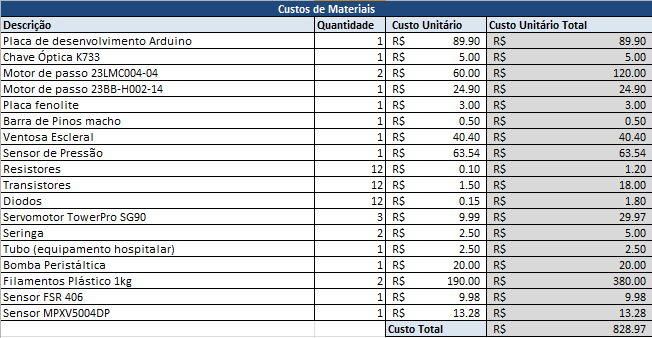
\includegraphics[scale=1.0]{figuras/customateriais.png}
		\caption{Custo dos Materiais}
		\label{customateriais}
\end{figure}


Com isso, o custo total do produto Posicionador de Lente seria de 828,97 reais, desconsiderande a margem de lucro a ser aplicada sobre esse valor.

O custo do projeto envolve investimentos não só nos materiais como também em mão de obra, equipamentos e softwares. O custos de equipamento, software e mão de obra são apresentados na figuras \ref{custoequip}, \ref{custosoft} e \ref{customao}, respectivamente.

\begin{figure}[H]
		\centering
			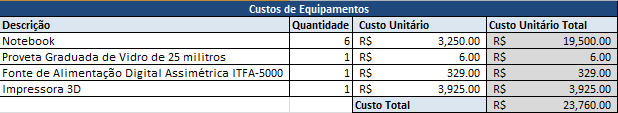
\includegraphics[scale=1.0]{figuras/custoequip.png}
		\caption{Custo dos Equipamentos}
		\label{custoequip}
\end{figure}

\begin{figure}[H]
		\centering
			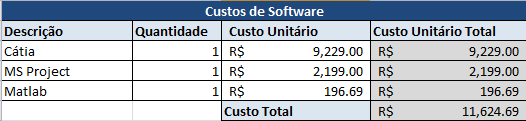
\includegraphics[scale=1.0]{figuras/custosoft.png}
		\caption{Custo dos Softwares}
		\label{custosoft}
\end{figure}

\begin{figure}[H]
		\centering
			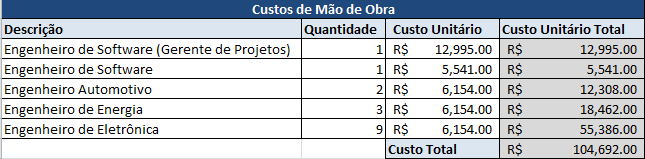
\includegraphics[scale=1.0]{figuras/customao.png}
		\caption{Custo de Mão de Obra}
		\label{customao}
\end{figure}

Com isso, apesar do custo do produto ser 828,97 reais, o investimento inicial para construir um protótipo do mesmo é de cerca de 140.905,66 reais conforme mostrado na figura \ref{investimento}.

\begin{figure}[H]
		\centering
			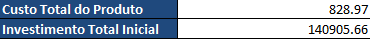
\includegraphics[scale=1.0]{figuras/investimento.png}
		\caption{Custo e Investimento Total}
		\label{investimento}
\end{figure}